%% Submissions for peer-review must enable line-numbering 
%% using the lineno option in the \documentclass command.
%%
%% Camera-ready submissions do not need line numbers, and
%% should have this option removed.
%%
%% Please note that the line numbering option requires
%% version 1.1 or newer of the wlpeerj.cls file, and
%% the corresponding author info requires v1.2

% \documentclass[fleqn,10pt,lineno]{wlpeerj}
\documentclass[10pt,lineno]{wlpeerj}
% \documentclass[10pt]{wlpeerj}
% \usepackage{cite}
\usepackage{amsmath,amssymb,amsfonts}
\usepackage{algorithmic}
\usepackage{graphicx}
\usepackage{booktabs} 
\usepackage{textcomp}
\usepackage{xcolor}
\usepackage{soul}
\usepackage{soulpos}
\usepackage[ruled,vlined]{algorithm2e}
\usepackage{graphicx}
\usepackage[switch]{lineno}
% \usepackage{lineno}
% \linenumbers
\usepackage{lipsum} 
\usepackage{pgfplots}
\usepackage{placeins}
\usepackage{float}
\usepackage{placeins}
\pgfplotsset{compat=1.18}
    
\title{X-Modalities Fusion using Contrastive Learning for Image Retrieval}
\author[1]{Ikhlaq Ahmed}
\author[1]{Naima Iltaf}
\author[1]{Usman Zia}
\author[2]{Zafran Khan}

\affil[1]{Department of Computer Software Engineering, National University of Sciences and Technology Islamabad (e-mail: iahmed.phdsemcs@student.nust.edu.pk ; naima@mcs.edu.pk, usman.zia@sines.nust.edu.pk)}
\affil[2]{School of Electrical Engineering and Computer Science, Gwangju Institute of Science and Technology (GIST), Gwangju, South Korea (e-mail: zafrankhan1830@gm.gist.ac.kr)}

\corrauthor[1]{Naima Iltaf}{naima@mcs.edu.pk}
 
\begin{abstract}
Image search with desired modification through text query holds promise for daily uses, including online shopping and surfing on the internet. The goal is to utilize set of integrated features of both the visual and corresponding textual query to retrieve images that align with the original image while incorporating the modifications detailed in the provided text description. This presents three key challenges. Firstly, the challenge lies in itself i.e; the misalignment between two completely different modalities of vision and text. Secondly, there is a need to make targeted modifications to specific attributes of the query image in accordance with textual descriptions. Another challenge arises when absence of contextual understanding is faced due in-appropriate structure or conceptual understanding of textual query. These challenges are notably intricate as they require a collaborative comprehension of both image and text modalities. This paper introduces a two stage framework that utilizes features extracted by Constrastive Language-Image Pre-trained (CLIP) model. Initially, CLIP encoders are aligned by combining visual and textual features through element-wise summation. The contextual understanding of the query is supplemented by introducing a Knowledge Embedded stream (KES) in the proposed framework. KES is utilized to integrate concepts into the textual query by leveraging the global features of the reference image. Subsequently, relational network is trained sequentially aimed to seamlessly combine features from both modalities. Thereby integrating bimodal information and generating unified features. These jointly learned features are then utilized for retrieval purposes. Contrastive learning is employed consistently in the training of both stages. The proposed framework has been evaluated using two real-world fashion domain datasets, Fashion-200K and Fashion-IQ, as well as the CIRR dataset, which consists of real-life images. Accordingly, results showed that it performed better than baseline frameworks used for comparative analysis.

\end{abstract}
 \maketitle
 
\begin{document}
\vspace{-3.0\baselineskip} % Reduce vertical space between subsections
\subsection*{}\textbf{Subjects}  Computer Vision, Natural Language Processing
\vspace{-1.8\baselineskip} % Reduce vertical space between subsections
\subsection*{}\textbf{Keywords} Contrastive Learning, CLIP, Visal and Textual features extraction, Image retrieval framework, Feature joint venture, Re-Ranking Algorithm.
\flushbottom
\maketitle
\thispagestyle{empty}

\section{Introduction} 
Image retrieval involves searching for images in a database that match a user's request. Generally such retrievals are on the basis of image to image \citep{Albert} and text to image \citep{Kuang} queries used for retrievals. These are single modality query based on visual or linguistic contents. At certain time, users desire to modify the query image according to their wishes expressed through text. Thus accurately grasping the user's intents to modify the image at particular region poses a considerable challenges, hindering retrieval systems from fully comprehending. To tackle this challenge, some researchers have proposed paradigms \cite{DenseBert4Ret,DvLIL,DM-RR,KSC-2023} that incorporate user feedback into the system to improve the quality of the retrieved content. 
\par Foregoing in view, rationale for this paper is that it handles the complexity of retrieving an image on the basis of an image query which is complemented with linguistic query by the user. Such provision gives freedom to the user to express his/her intentions to modify the query image. As illustrated in Figure \ref{fig:CBIR_Example}, it is aimed to find the target image aligned with a visual query modified by text input. The modified text specifies the attribute information that the user desires to alter in the visual query. These modified attributes encompass a diverse range, including color,texture and spatial domains. This scenario introduces a more intricate challenge of multi-modal composition, necessitating a homogeneous understanding of both the visual and textual query components.

\par Image retrieval based on dual modalities faced three intricate challenges that need to be catered for. Firstly, when entirely different modalities of textual and visual modalities are encoded, their encoded vectors falls apart in the embedding space, leading them to be disjoint set. This visual and textual features misalignment issue have been mitigated by employing CLIP’s visual and text encoders, which align both modalities by creating a unified embedding space. Another challenge being face with dual modalities based CBIR is the composition framework is to correlate the semantics of textual query to specific region of the reference image. The coherent working of relational network and CLIP encoders enforce the proposed model to comprehend the semantics of the textual query and correlate it to local region of the reference image. Lastly, the textual query often fails to provide the contextual and semantic richness required to clearly articulate the desired modifications to the query image. To enhance the contextual understanding of query to the proposed framework, we introduced a KES to capture the concept of query image and incorporate it into the text query. Hence, improving the contextual understanding of textual queries for a fair understanding of the model. 

 The challenges outlined in the paper and their solution can be directly linked with the example in Fig-\ref{fig:CBIR_Example}. The first challenge, misalignment between textual and visual modalities, arises as the term "cocktail dress + shoulder straps and red color" in the textual query needs to be accurately aligned with the query image. This is addressed by the use of CLIP encoders, which align textual and visual embeddings within a unified space. The second challenge involves correlating text semantics with specific visual regions, requiring the model to correlate the textual description of "cocktail dress + shoulder straps and red color" with the relevant regions of the reference image. This is achieved through the relational network, which effectively combines textual and visual features to establish these correlations.  Lastly, the third challenge concerns enhancing the contextual understanding of textual queries. For instance, the term "shoulder straps and red color" alone may lack sufficient context to fully convey the intended modification, but when enriched with the context "cocktail dress" the semantic intent becomes clear. The KES supplements the textual query with global context from the reference image, ensuring complete semantics and improving retrieval accuracy.  Together, these mechanisms enable the framework to address the challenges and retrieve the correct modified target image in alignment with the given example. \color{black} The key achievements of the proposed paradigm are outlined below: \color{black}

\begin{itemize}
   \item Devised a visio-linguistic pretrained encoding model that leverages contrastive learning to address cross modalities alignment issue in the common embeddings domain.
   \item Introduced a re-ranked based KES to enhance the contextual understanding of textual query aligned with reference image and to generate the most suitable textual queries against reference image.
   \item For cross modal relational understandings, a relational network that is tuned in conjunction of CLIP encoders and driven by the constrastively learned joint embeddings.  
  \item Comprehensive evaluation of two fashion domain datasets(Fashion-200K and Fashion-IQ) and a real life images dataset(CIRR) demonstrating the outperformance of the proposed framework.
\end{itemize}

\begin{figure}[t]
    \centering
      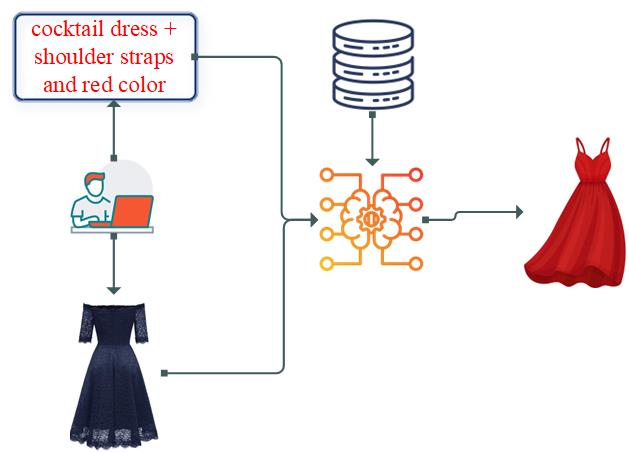
\includegraphics[width=1\columnwidth,height=65mm]{Fig-1.jpg}
        \caption{CBIR system in our daily life activities}
    \label{fig:CBIR_Example}
\end{figure}


% \par The section wise structure of the paper is as follows: Section \ref{sec:LR} delves into the relevant literature, while Section \ref{sec:proposed_methodology} presents a thorough elucidation of the proposed framework. The practical implementation, results, and ablation studies are detailed in Section \ref{sec:experimentation_and_results} and discussed in Section \ref{sec:Ablation_studies}. Ultimately, Section \ref{sec:conclusion} concludes the research and outlines potential avenues for future exploration.

\par The paper's structure is set out as outlined below: Section-\ref{sec:LR} provides an overview of the relevant literature, and Section-\ref{sec:proposed_methodology} provides a comprehensive explanation of the proposed paradigm. Section-\ref{sec:experimentation_and_results} covers the implementation, results, and ablation studies, with further discussion presented in Section-\ref{sec:Ablation_studies}. Finally, Section-\ref{sec:conclusion} wraps up the research and highlights potential directions for future research.

\section{Related Work}\label{sec:LR}
\par Image retrieval systems are commonly classified into two primary types: Text-Based and Content-Based. In a Text-Based system, the retrieval of images is driven by the tags or descriptions associated with each image. The process involves analyzing the text features of a user's query by comparing them with the metadata tags or annotations within the dataset. Following this, the system displays to the user, the most pertinent and analogous images determined from this comparison. A content-based image retrieval system organizes images based on their visual attributes, encompassing aspects like color, texture, contours, and the spatial configuration of objects within the image frames. In this system, retrieval revolves around comparing the visual characteristics of the images stored in the database with those of the query image.

Interactive image retrieval seeks to improve result accuracy by incorporating user feedback, often through attribute labels and modified text. In our study, we have concentrated on interactive image retrieval, specifically focusing on modified text as the primary feedback mechanism. Many studies address this challenge by integrating image and text components. For instance, in the TIRG \citep{Nam}, a residual gating module is introduced to aid in learning composite image-text representations. For deep visual features extraction , a deep convolutional neural network have been used by the AutoRet\citep{AutoRet1} framework from segmented portions of images, which are then grouped into distinct clusters, enhancing performance in content-based image retrieval tasks. After the embeddings have been obtained, the AutoRet framework applies a clustering algorithm to group embeddings with similar characteristics together. Every cluster corresponds to a collection of visually akin image patches. This clustering process holds significant importance in structuring the image data, streamlining procedures, and enhancing the retrieval of visually analogous images. The paradigm  “Attributes as Operators” \citep{Attributes_as_operators} introduces a technique for representing the visual characteristics of an entity through attributes. In this method, embedding of the model is trained and learned exclusively by considering the interpretations of the attributes associated with linked entities. In addition to real-valued methods, various hashing techniques have been extensively studied, especially for handling extensive datasets where efficiency in CBIR is critical. \cite{Deep_Hashing} proposed Deep Cauchy Hashing (DCH), which employs a Cauchy distribution-based loss function to boost retrieval accuracy. A self-attention-based model \cite{Transformer_Hashing} was also introduced, utilizing dual-stream feature learning to enhance the discriminative power of image hashing.

\par The Augmented Tirg method outlined in \citep{aug-tirg} improves upon the earlier TIRG framework \citep{Nam} by integrating ResNet with the model structure. This inclusion enables a more extensive fusion of image and text features. Similar to the initial TIRG framework, a straightforward gating mechanism is utilized in order to generate a unified feature embeddings of both the visual and textual data. In addition to feature extraction and joint representation, academic researchers have also explored re-ranking techniques to improve the performance of single-modality searching \citep{SMR-1, SMR-2, SMR-3, SMR-4}, object recognition \citep{OR-1, OR-2}, and textual query based image retrieval \citep{TQ-1, TQ-2, TQ-3} tasks. In these re-ranking approaches, the retrieval process is reciprocal, meaning that if an object embeddings from visual modality X is a potential match with embeddings from textual modality Y, the opposite holds true as well. Expanding on this idea, \citep{RR} presents a multivariate re-ranking algorithm that employs k candidates from the other modality to facilitate reverse retrieval. This approach amalgamates diverse bidirectional retrieval parameters to optimize the retrieval outcomes. Likewise, \citep{SMR-2} proposes a bidirectional ranking method that iteratively calculates reciprocal similarity. Utilizing the bidirectional nature of the retrieval process and incorporating it into re-ranking algorithms, researchers have sought to improve the overall retrieval performance, making it more efficient and accurate for various tasks involving diverse modalities. The DQU-CIR \cite{DQU_CIR_Rev2} framework generates unified textual and visual queries from raw data of multimodal input, utilizing BLIP-2 and LLM, respectively. The textual query is encoded using the Vision-Language Pre-trained Model (VLPM) textual encoder, while the visual query is embedded through the VLPM vision encoder. These extracted features are then fused using a multi-layer perceptron. DQU-CIR has been evaluated with four datasets, including three from the fashion domain and another from the real-life domain. The TG-CIR \cite{TG_CIR_Rev3} framework operates in three distinct stages. In the first stage, it extracts both high-level and detailed features from the source image, target image, and input text using VLPM's visual and textual encoders. To enhance generalization and reduce inter-dependency among the queries, orthogonal regularization is applied. In the second stage, the framework utilizes the concept of transfer learning aimed at learning multimodal queries autonomously. This helps the student model resolve conflicts between the source image and the modification text, thus improving overall query composition and retrieval. In the final stage, TG-CIR incorporates two types of losses to refine its performance: the conventional batch-wise classification loss and batch-wise target similarity-guided matching loss to enhance the model's ability to aptly rank retrieved images. For model evaluation, the TG-CIR approach utilized fashion-related datasets along with a real-life image dataset.

\par In contrast, our proposed approach begins with the fundamental concept of establishing an shared embedding space for both visual and textual contents. Such embedding space is generated using vision-language model, namely CLIP\citep{CLIP}. Initially, the visual and linguistic encoders of the CLIP are trained, specifically for image search using joint vision-text queries. Subsequent to the alignment of the CLIP encoder, we employ these aligned encoders to train a follow-up relational network, to effectively merge the features of dual modalities and establish strong correlations between the text query semantics and particular regions of the query image. Moreover, to enhance the contextual understanding of query, we introduced a RR(Re-ranking)\cite{RR,GalR,DM-RR,Pic2Word} based version of KES \cite{BKP} to capture the concept of query image and incorporate it into the text query. Hence, improving the contextual understanding of textual queries for a fair understanding of the model. \color{black}

\section{Proposed Methodology}\label{sec:proposed_methodology}
The proposed paradigm addresses three critical challenges in composed image retrieval. The first challenge, aligning textual and visual features, is tackled using CLIP. The CLIP visual encoder extracts rich visual embeddings from the query image, while the language encoder generates meaningful representations from the textual queries, ensuring alignment between the textual and visual domains. These aligned encoders are further utilized to train a relational network, enabling the effective fusion of dual-modality features and establishing strong correlations between the semantics of the textual query and the local regions of the query image. The integrated features are undergo a two-stage framework where element-wise summation combines the modalities, and contrastive loss ensures that image-text pairs are tightly aligned in the embedding space while remaining distinct from non-matching pairs. 


To address the third challenge of improving the contextual understanding of textual queries, we incorporate the Knowledge-Embedded Stream (KES), drawing inspiration from the work of \cite{BKP}. This component enriches relative captions by embedding contextual and semantic information derived from the attribute information of the query image. By providing additional contextual depth, KES ensures that the textual query reflects the necessary modifications with semantic and contextual completeness. This enhancement not only improves alignment between the textual and visual queries but also establishes a robust connection between the enriched textual semantics and specific regions of the reference image, thereby enhancing the accuracy and relevance of retrieval results.

The presented method addresses the complexity of multi-modal composed image retrieval. It functions by processing a joint query that is composed of a query image $I_r$ (like an image of a woman's shirt with full sleeves) and a corresponding textual amendments $T_r$ containing a user's descriptive request about the modifications in image (for example, "woman's shirt + is solid black with no sleeves"). The objective is to retrieve an image that meets the criteria set by the combined query, such as an image depicting a sleeveless shirt in black color, as depicted in Fig. \ref{fig:proposed_framework}. To achieve successful retrieval of target image, the CBIR system needs to comprehend the semantic content of textual query, interpret the visual features of reference image, integrate information from both the modalities(visual and textual), and subsequently employ the merged representation to identify relevant images.

In contrast to the earlier studies, which rely on various models for processing images and text separately, the proposed framework is entirely focused on formulation of a joint representation for both the image and text queries. 
The creation of a unified embedding is accomplished by leveraging the CLIP \citep{CLIP} model, a visual linguistic model that is primarily proposed and developed to align visual features against their related textual annotations within a shared embedding space. Prior to creation of the joint representation, the textual query has been enhanced with global features of the reference image  using KES.   

The CLIP framework comprises of two fundamental encoders: one designed for processing images (denoted as $\mathcal{E}_i$) and another tailored for handling textual data (represented as $\mathcal{E}_t$). The main function of a visual encoder is to generate feature patterns $\mathcal{E}_i(I) \in \mathbb{R}^D$ for an image I. Likewise the encoder for textual data produces an embedding $\mathcal{E}_t(T) \in \mathbb{R}^D$ for given text query T. Here, D refers to the space in which the visual and textual features are represented.

The training process of CLIP is designed to ensure that similar concepts conveyed through images and text are mapped to closely related feature representations. For example, considering an image of a dress labeled as $I_d$ and a corresponding textual description $T_d$ like "a photo of a dress," the CLIP training methodology ensures that $\mathcal{E}_i(I_d) \approx \mathcal{E}_t(T_d)$.
% \color{red}

We argue that while a unified embedding space serves as a robust foundation, it may not precisely address the particular needs of the task at hand. In the realm of image retrieval utilizing joint queries, the goal is to navigate through an embedding space, moving from the reference image towards the corresponding target image. This transition is guided by the knowledge base textual query. Thus, rather than depending on a single image-text embedding space, the proposed framework involves establishment of two separate embeddings that can be a joint ventured through a summation.

 To formalize this, consider an image $I_x$ portraying a shirt with full sleeves and the corresponding text $T_y$("woman's shirt + is solid black with no sleeves") used to modify $I_x$ . The relative caption $T_y$ has been enhanced with the help of a Knowledge-Embedded Stream (KES), enriching the textual query with additional contextual and semantic depth of the reference image, ensuring it captures the conceptual modifications. Let, $I_z$ denotes a sleeveless shirt with black color. The goal is to configure these feature spaces in a manner that:

\begin{equation}
    \centering
    \mathcal{E}_i(I_x) + \mathcal{E}_t(T_y) \approx \mathcal{E}_i(I_z)
\label{eq:E_i}
\end{equation}

Both the textual and vision embedding space demonstrates "additive characteristics" in embedding plan, subject to satisfaction of Equation \ref{eq:E_i}.  It can be understood from Equation \ref{eq:E_i}, that textual query's embeddings supplemented with concept of the reference image through KES has the intuition of displacement vector from input reference image to target image. Such intuition can be deduced from rewriting Equation \ref{eq:E_t}.

\begin{equation}
    \centering
    \mathcal{E}_t(T_y)  \approx \mathcal{E}_i(I_z) - \mathcal{E}_i(I_x)
\label{eq:E_t}
\end{equation}

In order to obtain a target image using a combined input query, we leveraged the capabilities of CLIP's encoders via a two-step process. Initially in the first stage, we aligned the CLIP visual and textual encoders to learn through contrastive learning methodology that is specifically tailored for subsequent retrieval tasks. Moreover, pseudo-word tokens in the form of a concept have been generated using KES. The KES stream is designed to enhance text query embeddings by incorporating attribute information of the query image.
The second stage is about utilizing the contrastive features acquired in the first stage to train a relational neural network from scratch. This network is designed to effectively integrate image-text features at a fine-grained level. Despite training the relational network from the ground up, its architecture was meticulously designed to maximize the benefits obtained from the initial training stage.

During the inference phase, upon receiving a query $q = (I_q, T_q)$, we leverage the already fine-tuned encoders of CLIP aided with trained relational network module to produce the joint features. Employing the conventional image-image retrieval methodology, cosine distances are calculated among joint query and target image features stored in database. Subsequently, the retrieved results are organized and ranked based on similarity. The efficiency of the suggested approach is showcased in the qualitative results section, as illustrated in Figure-\ref{fig:QR}.

\subsection*{CLIP Encoders Alignment}\label{sec:Clip_Encoders}
In this stage, CLIP's visual and textual encoders are adjusted to enhance CBIR and reduce the disparity. The framework is provided with a visual query $I_q$ and a relative descriptive caption $R_c$. The relative caption is enriched with a improvised KES stream  as shown in Figure-\ref{fig:KES}. The primary goal of KES is to extract detailed attribute information in the form of pseudo-word tokens for subsequent integration in relative captions in place of an indicated place holder. Based on query image similarity, the top K=15 image-caption pairs are initially retrieved from a knowledge base randomly constructed from the training set. These pairs are further refined using re-ranking (RR) method, thereby selecting the top 5 most relevant image-caption pairs aginst earlier 15. The Top-K image and caption features provide deep contextual insight for mapping. Therefore, the contextual knowledge requested is fused with the features of the image query through a simple linear network $M_l$ to bring all the modalities to a common embedding space. The visual query features are then used to engage with the retrieved visual and caption features, using two separate inter-attention blocks $B$ to improve contextual comprehension and facilitate better interaction linking the reference image with the retrieved features. 
The resulting output $O$ is formed by concatenating three tokens: the mapped query image feature token $v' = M_l(v)$, along with two context-aware mapped tokens $O_v$ and $O_c$. This process can be written as:

\begin{equation}
    O_v = \text{B}(v', M_l(\{i_r^k\}_{k=1}^K), M_l(\{i_r^k\}_{k=1}^K))
\label{eq:vi}
\end{equation}

\begin{equation}
    O_c = \text{B}(v', M_l(\{t_r^k\}_{k=1}^K), M_l(\{t_r^k\}_{k=1}^K))
\label{eq:vi}
\end{equation}

\begin{equation}
    \centering
    O = \text{Concat}(v', O_v, O_c)
\label{eq:O}
\end{equation}

After generating the final output $O$, we adopt contrastive loss to train a mapping network enabling the textual features into the image embedding space against the image features.

We obtain the feature representations of visual query $I_q$ and KES-enriched relative descriptive caption $T_q$ by employing the visual ($\mathcal{E}_i$) and the textual($\mathcal{E}_t$) encoders of the CLIP respectively. This renders $\mathcal{E}_i(I_q)$ and $\mathcal{E}_t(T_q)$ $\in R^D$, with D representing the dimensionality of the features space of CLIP encoders. For a combined query formulation, element-wise summation is performed as:

\begin{equation}
    \centering
    \theta_q  = \mathcal{E}_i(Iq) + \mathcal{E}_t(Tq)
\label{eq:theta_q}
\end{equation}
Our objective comprises two main aspects: Firstly, to minimize the distance separating the integrated features of the query, represented as $\theta_q$, and the target image features, denoted as $\theta_t = \mathcal{E}_i(I_t)$, within the same triplet. This aims to place the features of $\theta_q$ and $\theta_t$ in close proximity within the embedding space. Secondly, to maintain a separation between $\theta_q$ and other target images. To accomplish this, we utilize batch contrastive loss, as depicted in Equation \ref{eq:Contrastive_Loss}:

\begin{equation}\label{eq:Contrastive_Loss}
- \frac{1}{N} \sum_{i=1}^{N} \log \frac{e \left(\operatorname{sim}\left(\theta_q^i, \theta_t^i\right) / \tau\right)}{e \left(\operatorname{sim}\left(\theta_q^i, \theta_t^i\right) / \tau\right)+\sum_{j=1}^{N} e \left(\operatorname{sim}\left(\theta_q^i, \theta_t^j\right) / \tau\right)}
\end{equation}

In this equation, $\operatorname{sim}\left(\theta_q^i, \theta_t^i\right) / \tau$ represents the cosine similarity with $\tau$ as a temperature scale for logits control. Moreover, $N$ is the total images in one batch to which the contrastive loss is applied for fine tuning of encoder's weight. We used batched contrastive loss as it eliminates the need of sampling strategy; considering all $-ve$ samples within a micro batch. Tailoring and tuning of both visual and textual encoders are illustrated in Figure-\ref{fig:proposed_framework}. 
Moreover, Table-\ref{tab:notation_table_fig2} presents a comprehensive list of all the notations along with their descriptions used in Figure-\ref{fig:proposed_framework}.

\begin{figure*}[t]
    \centering      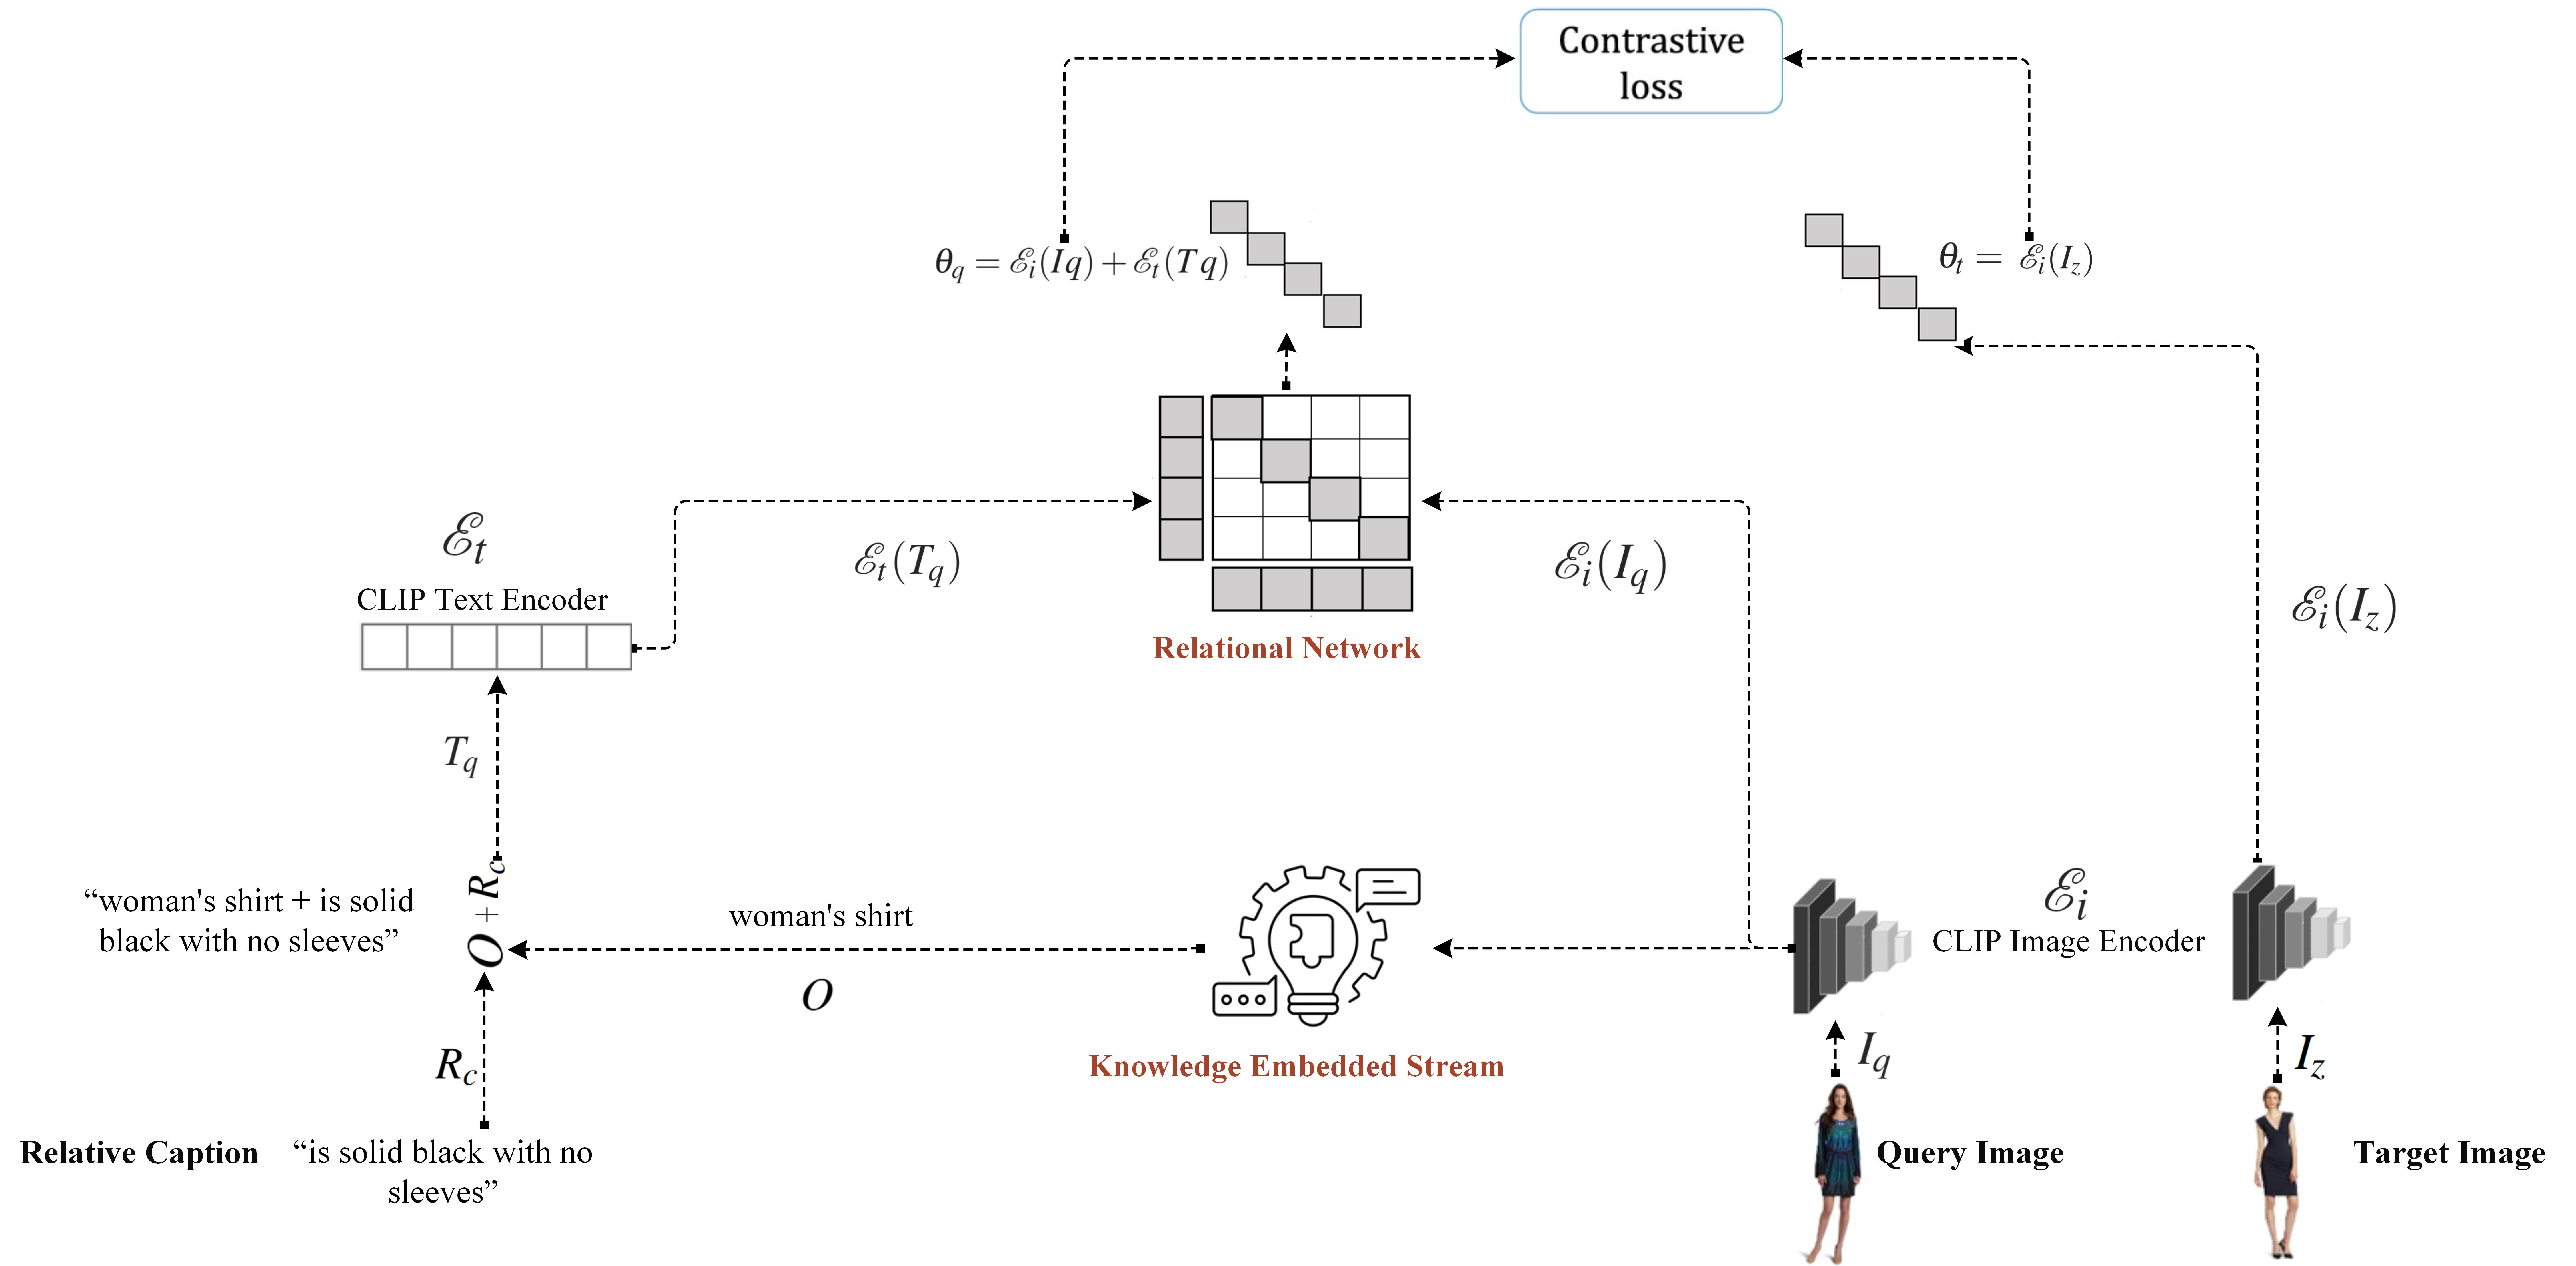
\includegraphics[width=0.75\textwidth,height=75mm]{CLIP_Encoders_Alignment.jpg}
        \caption{CLIP Encoders Alignment: Features from both image and text CLIP  encoders are combined via element-wise summation , and subsequently its refinement with target image features using batch contrastive loss.}
    \label{fig:proposed_framework}
\end{figure*}

\begin{table}[h!]
\small
\centering
\begin{tabular}{|c|l|}
\hline
Symbol & Description \\ \hline
 $T_q$ & Text Query \\ \hline
 $I_q$ & Image Query \\ \hline
 $I_z$ & Target Image \\ \hline
 $\mathcal{E}_t$ & Text Encoder \\ \hline
 $\mathcal{E}_i$ & Image Encoder \\ \hline
 $\mathcal{E}_t(T_q)$ & Text Query Generated Features \\ \hline
 $\mathcal{E}_t(I_q)$ & Image Query Generated Features \\ \hline
 $\mathcal{E}_t(I_z)$ & Target Image Generated Features \\ \hline
 $\theta_q  = \mathcal{E}_i(Iq) + \mathcal{E}_t(Tq)$ & Element-Wise Summation \\ \hline
 \end{tabular}
\caption{Notation Table}
\label{tab:notation_table_fig2}
\end{table}
\FloatBarrier
\begin{figure*}[t]
    \centering      \includegraphics[width=0.75\textwidth,height=75mm]{KES.jpg}
        \caption{Architecture of the Knowledge-Embedded Stream (KES): Enriching Textual Queries with Contextual and Semantic Features Derived from Reference Image.}
    \label{fig:KES}
\end{figure*}
% 
\FloatBarrier

The summation of individual modalities, element by element, aligns with the additive property of the embedding space produced by CLIP encoders. This reflects the fact that text and vision modalities do not share an identical feature space; rather, the text modality acts as a displacement vector, representing the shift from the visual query to the desired target image. However, the absence of sufficient contextual information can further displace these modalities, widening the gap between them. This challenge is addressed through the incorporation of the Knowledge-Embedded Stream (KES), which enriches the contextual and semantic depth of the textual modality, ensuring a more cohesive alignment and correlation between the two modalities.

Adopting a broader view, it is noticed that in image retrieval, using dual modality, both the individual query modalities do not play identical role. This lacks symmetry in terms of sequential inputs. Such as it starts with an input query image which aims to get target image using textual query guidance. Thus, the partitioning of the unified embedding space is an intentional design choice that is aligned with the intrinsic nature of the retrieval task. From this point onward, we will utilize the notations $\tilde{\mathcal{E}_i}$ and $\tilde{\mathcal{E}_t}$ to show aligned CLIP image and text encoder, respectively.

\subsection*{Relational Network Tuning}\label{sec:Clip_Encoders}
Regarding Relational Network training, we adhere to the identical philosophy as we did earlier. However, a different strategy is employed by training from scratch rather than just adjusting the weights of both visual and textual encoders. Unlike the initial stage, we utilize the relational network, represented as $R_\theta$, to construct the joint query. More precisely, we obtain the combined features as follows.

\begin{equation}
    \centering
    \tilde \theta_q = R_\theta(\tilde{\mathcal{E}_i}(I_q),\tilde{\mathcal{E}_t}(T_q))
\label{eq:thetha_q}
\end{equation}

% $L_{gpt}$

To optimize the relational network, we use the $L_{contr}$ loss described in Equation \ref{eq:Contrastive_Loss}, with $\tilde\theta_q$ and $\tilde\theta_t = \tilde{\mathcal{E}_t}(I_t)$ as inputs. Through the application of the contrastive loss, we aim to optimize the training of the network $R_{\theta}$ for features generations that closely match the target features while ensuring a substantial separation from all other image features.

The architectural design of the relational network, as illustrated in Figure \ref{fig:RN_framework}, is purposeful in harnessing the benefits obtained during the initial training phase. Its fundamental concept is centered on comprehending the residual of a convex combination among the query features of individual modalities (vision and text).

The process commences by application of linear transformation to both the text and image modalities features, followed by the application of a ReLU activation function. Following this, the projected embeddings obtained are concatenated and then forwarded through two distinct channels. In Figure \ref{fig:RN_framework}, the branches on either side are responsible for determining the coefficients for the convex combination of both the individual modality features. To have these coefficients, these features undergo a series of sequential operations, including a linear,ReLU, and lately a sigmoid function. The output of the sigmoid yields the proper parameters for the convex amalgamation of the query characteristics for each modality separately. The alternative branch, positioned in the middle of Figure \ref{fig:RN_framework}, computes the proportionate of each modality feature to the joint venture. Its structure closely mirrors that of the first chanel, with the exception that it lacks the final sigmoid activation function.

Finally, individual query features and learned text-image feature were summed up. Dropout with the rate of $0.2$ is implemented to avoid over-fitting. $\sigma$ and $(1 - \sigma)$ indicating the output of first and second channel, the combined features can be expressed as:

\begin{equation}
    \centering
    \tilde\theta_q = (1 - \sigma)\tilde{\mathcal{E}_i}(I_q) +\sigma\tilde{\mathcal{E}_t}(T_q) + \lambda
\label{eq:thetha_q_comb}
\end{equation}
It is crucial to emphasize that the convex combination is the generalization of element by element summation of the joint query characteristics. This rendered the additive properties of embedding space with enhanced effectiveness of the tuned relational network. The design of the said network intentionally harnesses the task adaptation acquired in the initial training stage.

\begin{figure*}[t]
    \centering
      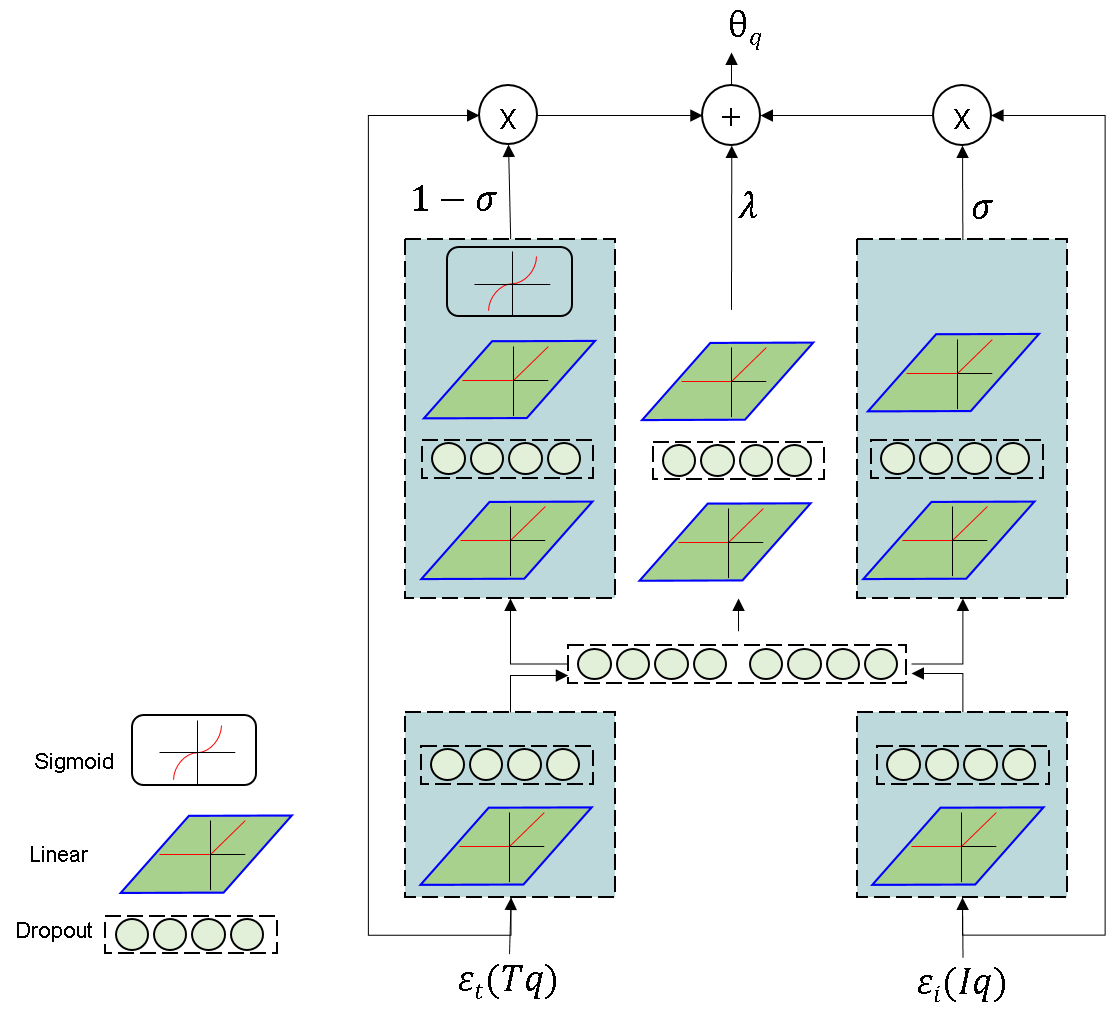
\includegraphics[width=1\textwidth,height=100mm]{Integrator.jpg}
        \caption{Relational Network}
    \label{fig:RN_framework}
\end{figure*}
\FloatBarrier

\color{black}

\section{Experimental setups and Results}\label{sec:experimentation_and_results}
\subsection*{Implementation details}

In our experiments, during first stage of proposed model, we utilized the CLIP model based on modified ResNet-50 architecture \citep{CLIP}. It processes images with dimensions 224 and the embedding space is configured to be of dimension D = 1024.
During second stage network, illustrated in Figure-\ref{fig:RN_framework}, input of the first two linear layers is set to D, while the output dimension is 4D. Following the concatenation of outputs from both the channels, it undergoes processing through two more linear layers. The initial linear layer of 1st channel has an input size of 4D and output of 8D. The second one has an input dimension of 8D with the output dimension set to 1. In the second channel, the input-output dimensionality of of first linear layer is set to (4D, 8D), while the second linear layer has dimensions (8D, D). Following standard procedures, a dropout rate of 0.5 is implemented. In the process of retrieval, both the integrated features and those in the index set are normalized to attain a unit L2-norm.

Consistent with the inherent CLIP learning methodology, we opted for the AdamW optimizer, configuring the LR(Learning Rate) to $2e-6$, and the WDC(Weight Decay Co-Efficient) to $1e-2$. Additionally, for logits to have an ample dynamic range, we set $\tau = 100$ in Equation \ref{eq:Contrastive_Loss}. To accommodate GPU memory limitations, we adjusted the batch size to 64. We maintained the batch normalization layer in a frozen state, preventing it from being updated and conducted the tuning for maximum 100 e-pochs. 

While training the Relational network, the weights of the CLIP encoders were kept unchanged from the initial stage. For this phase, a learning rate of $2e-5$ was utilized, with training executed for up to 100 iterations(epochs) and a batch comprising 128 samples. The framework was implemented on a 64-bit Ubuntu Long-Term Support operating system with 32GB of memory (RAM) and an eight-core AMD processor. The system featured an NVIDIA 3090Ti GPU with 12GB of memory. To address Cuda out-of-memory issues, 60GB of swap memory was utilized.

\subsection*{Datasets}
The proposed framework have been evaluated using two real world fashion domain datasets, Fashion-200K and Fashion-IQ, as well as the CIRR dataset, which consists of real-life images. All of the three datasets are widely recognized within the research community for facilitating CBIR tasks.

The FashionIQ dataset comprises 77,684 fashion images, divided into training, validation, and test sets. Three unique classesi.e. dress, shirt and are used to organize these images. It was observed that many image links are broken, rendering the corresponding images inaccessible. To maintain robust training, the missing images of the dataset are excluded. In the training set, each triplet consists of a query image, two related textual descriptions, and a matching target image. These textual descriptions specify the visual changes required for the query image to resemble the desired target image. Similarly, the Fashion200k dataset includes a wide range of fashion-related images, with approximately 200,000 entries. Each image in this dataset is paired with a textual description detailing its attributes. The CIRR dataset, designed for Compose Image Retrieval on Real-life Images, comprises 21,552 genuine real-world visuals derived from the NLVR2 \cite{CIRPLANT} dataset. It includes 36,554 triplets, with 80\% allocated to training, and 10\% each to validation and testing. The images are organized into collections of six, with each collection sharing both visual and semantic similarities. The dataset's captions emphasize the distinctions among images within the same group, increasing the complexity of the retrieval task as it requires identifying subtle differences between closely related images.

\subsection*{Evaluation Metrics}
\par The evaluation procedure follows the standard experimental setup outlined in the literature. The primary metrics used for model evaluation are Recall at rank K (R@K), with particular emphasis on K = {5, 10, 50}. It is important to note that each triplet includes a single positive image, meaning each bi-modality query can have at most one positive match, or none, within the Recall@K metric.

\subsection*{Quantitative analysis}
Following established academic research practices in the field, the proposed model has undergone evaluation using the metric known as "Recall@K," denoted as Recall at K. In the field of CBIR, Recall at K refers to the proportion of images accurately retrieved within the top-K results during a dual-modality search. This evaluation metric measures the fraction of accurately identified images relative to all the retrieved images. To enable a quantitative comparison between the proposed model and established baselines in the CBIR domain, we have outlined the following methodologies based on our current understanding:

\begin{itemize}
   
    \item Relationship\citep{relationship}: 
This method incorporates the use of a Relational Network (RN) designed for complex reasoning, capable of managing both text-based and visual queries. Convolutional Neural Networks (CNNs) are employed to fetch bi-dimensional visual features and transform them into relational representations. The extracted visual embeddings are subsequently combined with textual data by leveraging their underlying relationships. The combined relational information is further processed through a Multi Layered Perceptron (MLP), and the averaged output are utilized to develop a model proficient in handling both textual and visual inputs.
    %(Santoro \emph{et al.})
    \item FiLM (Feature Wise Linear Modulation) \citep{film}: In this approach, the embedding layer of the Convolutional Neural Network (CNN) is provided with information from both the visual and textual components. By simultaneously incorporating both aspects, the transformed feature space is projected, which is subsequently utilized to alter the features of an image. This method primarily focuses on improving effectiveness in the area of VQA(Visual Question Answering). %(Perez \emph{et al.})
    \item TiRG\citep{Nam}:  The approach known as Text-Image Retrieval Gating, abbreviated as TIRG, involves the simultaneous learning of visio-linguistic features and the composition of their representations. The approach harnesses Convolutional Neural Networks (CNNs) to fetch visual features and utilizes Long Short-Term Memory (LSTM) for generating textual features. To achieve a joint representation, TIRG employs a gating mechanism that blends the textual and visual features together.
    \item ComposeAE\citep{ComposeAE}:   
    This work presents an autoencoder-based model aimed at learning the composition of visio-linguistic queries for image retrieval. The framework employs ResNet-50 for extracting image features and BERT for extracting text features. By leveraging a deep metric learning approach, it learns a metric that minimizes the gap between the combined representation of the source Visio-Linguistic query and the target images.
    \item MRN\citep{MRN}: 
MRN effectively captures joint representations from both visual and textual data by using element-wise multiplication of joint residual mappings. This method draws on concepts from attention-based models.
    \item CIRPLANT\citep{CIRPLANT}: 
    This approach introduces a transformer-based framework utilizing extensive pre-trained V\&L (Vision and Language) insights to adapt visual embeddings based on linguistic conditions. Information search is carried out by conducting a NN(Nearest Neighbor) search on the adjusted embeddings.
    \item VAL \citep{VAL}: 
    The Visiolinguistic Attention Learning (VAL) framework presents a composite transformer integrated seamlessly with a Convolutional Neural Network, It specifically preserves and modifies image characteristics based on textual embeddings. Through the inclusion of multiple composite transformers at various depths, VAL captures multi-granular visiolinguistic information, yielding a comprehensive representation for efficient image search.
    \item CosMo \citep{CoSMo}: 
    The Content-style modulation framework consists of two key modules based on deep neural networks.The first module i.e; content modulator makes local adjustments to the query image's features after normalizing its style. Subsequently, the style modulator injects global style information back into the modified feature.
    \item ACNet \citep{ACNet}: 
This work introduces a new Network, which consists of two main components. The MAM (Modality Alignment Module) aligns embeddings across various modalities using a contrastive loss between image and text. The RCM creates associations between image regions and their corresponding textual descriptions, adaptively adjusting specific regions of the query image based on the semantic content of the text.
    \item CLVC-Net \citep{CLVCNet}: 
This framework introduces two unified modules: the fine-grained local composition module and the fine-grained global composition module, designed to address complex multi-modal compositions. Furthermore, a mutual enhancement module facilitates the exchange of knowledge between the local and global composition processes. 
   \item AACL \citep{AACL}:
Presents a novel method to address the challenge CBIR. The framework utilizes a multi-modal transformer architecture to effectively capture and represent the contexts of both image and text.
    
    \item RTIC \citep{RTIC}: Presents an architecture designed specifically for the image-text composition task, showcasing its effectiveness in encoding the differences between source and target images based on the provided text. Additionally, joint training technique is used that leverage graph convolutional networks, applied to any pre-existing composition methods in a plug-and-play fashion.
    \item Mix-Transformer \citep{Mix_Trans}: 
Proposes the integration of multi-headed self-attention (MSA) within the Vision Transformer (ViT) to focus on correlations among samples. It introduces the Group External Attention (GEA) module, replacing MSA in ViT with this module, leading to the development of the Mix-Transformer to enhance the effectiveness of the CBIR framework.

    \item CLIP4CIR \citep{CLIP4CIR_Rev2}: The proposed paradigm leverages the CLIP as the foundational vision-language pre-trained (VLP) model for extracting image and text features. After successful feature extraction it uses Combiner network to merge visual and textual features. For training loss the framework uses batch wise contrastive loss between the target and the fused features for parameters tuning. The CLIP4CIR have evaluated the approach on fashion-related dataset i.e; Fashion-IQ,Fashion-200K and CIRR dataset which is a real life time images. It is important to mention that great performance is achieved by CLIP4CIR, even with its simple architecture.

\item MAAF \citep{MAAF}:
   The MAAF approach extracts the image tokens through ResNet50 layers and combined it with text tokens extracted through LSTM. These tokens are stacked, and scaled dot-product attention is applied, followed by average pooling of the output for final representation.

   \item ARTEMIS \citep{ARTEMIS}:
   The text modifier is tokenized into individual words and then transformed using GloVe embeddings. A BiGRU or LSTM is subsequently employed, along with average pooling and a dense layer, to generate a feature representation at the sentence level. The image features are derived using a CNN with GeM pooling, followed by a newly learned fully-connected layer to further process the output.
 
\end{itemize}
We hypothesis that optimizing the text and image encoders leads to the acquisition of different and complementary information, which makes a distinctive contribution to enhanced performance.
We postulate that adjusting the image encoder primarily refines the image manifold, to better align with the fashion domain and real life images in our case. Conversely, aligning only the text encoder with the image query may not sufficiently fine-tune the language feature space for target image retrieval. To achieve better alignment of the text encoder, global and attribute information of the reference image has been integrated into the textual query using KES, enhancing the contextualization and semantic richness of the relative caption. This entails converting textual characteristics into displacement vectors in the image embedding space so as to enable more efficient retrieval using textual guidance. The quantitative outcomes of the proposed method for the Fashion-IQ, Fashion-200K, and CIRR datasets are assessed using Recall@K, are shown in Table-\ref{tab:fashioniq_results}, Table-\ref{tab:fashion200K_results}, and Table-\ref{tab:CIRR_results} , respectively.

It is evident that the two-stage approach, combining contrastive learning with CLIP-based feature extraction, outperforms its predecessors. The exceptional effectiveness of the proposed paradigm is due to its deep feature extraction capabilities, the distributed learning semantics associated with text queries, and the integration of the Knowledge-Embedded Stream (KES). KES plays a pivotal role by enriching textual queries with contextual and semantic depth, ensuring more precise alignment and correlation of textual features with the visual feature space, which significantly enhances the retrieval accuracy. The introduction of a relational network in the second stage for combined feature generation seamlessly connects textual modifications to their corresponding images within the trained embedding space. 
In this context, textual features operate as vectors within the visual feature space, ultimately converging the reference image towards the target image.
This results in a harmonious amalgamation of visual and textual characteristics. To demonstrate the proof of convergence of the model, its recall at K is plotted against epochs in parallel with the loss, as shown in Figure-\ref{fig:Fashion_IQ_Convergence} , Figure-\ref{fig:Fashion200K_Convergence} and Figure-\ref{fig:CIRR_Convergence} \color{black} for FashionIQ, Fashion200K and CIRR datasets respectively.

\subsection*{Qualitative Analysis}
The qualitative results emphasize the performance of our suggested two-stage paradigm. The retrieval examples in Figure-\ref{fig:QR} demonstrate the recall of the top 10 images, ordered based on their similarity scores with the reference image and its corresponding caption from the three datasets i.e; Fashion-IQ, Fashion-200K and CIRR. Along with leveraging CLIP's visual and textual encoders for feature extraction, our model incorporates the Knowledge-Embedded Stream (KES) to generate enriched, contextually robust, and semantically aligned embeddings for the reference image. 
These enhanced semantic and attribute representations are integrated into the relative caption, enabling more precise retrieval of the ground truth images. Figure-\ref{fig:QR} illustrates the reference image and relative caption, highlighted in blue and black, respectively. The pseudo-tokens generated by the Knowledge-Embedded Stream (KES) serve as placeholders within the textual query, providing more contextually robust and semantically enriched feature embeddings. The retrieved candidate images displayed on the right are arranged in descending order of similarity scores, starting with the highest similarity on the left and progressively decreasing toward the right. The target image is emphasized with a green border and zoomed in for better clarity, while the other images are framed with a red outline.

% \FloatBarrier

\begin{table}[htbp!]
\centering
\resizebox{\textwidth}{!}{%
\begin{tabular}{|c|cc|cc|cc|}
\hline
Frameworks    & \multicolumn{2}{c|}{Dress}         & \multicolumn{2}{c|}{Shirt}         & \multicolumn{2}{c|}{Toptee}        \\ \hline
              & \multicolumn{1}{c|}{R@10}  & R@50  & \multicolumn{1}{c|}{R@10}  & R@50  & \multicolumn{1}{c|}{R@10}  & R@50  \\ \hline
Relationship-\cite{relationship} & \multicolumn{1}{c|}{15.44} & 38.08 & \multicolumn{1}{c|}{18.33} & 38.63 & \multicolumn{1}{c|}{21.10} & 44.77 \\ \hline
MRN-\cite{MRN}        & \multicolumn{1}{c|}{12.32} & 32.18 & \multicolumn{1}{c|}{15.88} & 34.33 & \multicolumn{1}{c|}{18.11} & 36.33 \\ \hline
FiLM-\cite{film}          & \multicolumn{1}{c|}{14.23} & 33.34 & \multicolumn{1}{c|}{15.04} & 34.09 & \multicolumn{1}{c|}{17.30} & 37.68 \\ \hline
TIRG-\cite{Nam}          & \multicolumn{1}{c|}{14.87} & 34.66 & \multicolumn{1}{c|}{19.08} & 39.62 & \multicolumn{1}{c|}{18.26} & 37.89 \\ \hline
ComposeAE-\cite{ComposeAE}     & \multicolumn{1}{c|}{14.03} & 35.10 & \multicolumn{1}{c|}{13.88} & 34.59 & \multicolumn{1}{c|}{15.80} & 39.26 \\ \hline
CIRPLANT-\cite{CIRPLANT}     & \multicolumn{1}{c|}{17.45} & 40.41 & \multicolumn{1}{c|}{17.53} & 38.81 & \multicolumn{1}{c|}{21.64} & 45.38 \\ \hline
VAL-\cite{VAL}           & \multicolumn{1}{c|}{21.12} & 45.19 & \multicolumn{1}{c|}{21.03} & 43.44 & \multicolumn{1}{c|}{25.64} & 49.49 \\ \hline
RTIC-\cite{RTIC}         & \multicolumn{1}{c|}{27.38} & 52.95 & \multicolumn{1}{c|}{22.03} & 45.29 & \multicolumn{1}{c|}{27.33} & 53.60 \\ \hline
AACL-\cite{AACL}         & \multicolumn{1}{c|}{29.89} & 55.85 & \multicolumn{1}{c|}{24.82} & 48.85 & \multicolumn{1}{c|}{30.88} & 56.85 \\ \hline
CosMo-\cite{CoSMo}         & \multicolumn{1}{c|}{25.64} & 50.30 & \multicolumn{1}{c|}{24.90} & 49.18 & \multicolumn{1}{c|}{29.21} & 57.46 \\ \hline
ACNet-\cite{ACNet}        & \multicolumn{1}{c|}{29.20} & 55.68 & \multicolumn{1}{c|}{25.12} & 47.75 & \multicolumn{1}{c|}{30.96} & 57.72 \\ \hline
CLVCNet-\cite{CLVCNet}        & \multicolumn{1}{c|}{28.85} & 56.07 & \multicolumn{1}{c|}{28.75} & 54.76 & \multicolumn{1}{c|}{33.50} & 64.00 \\ \hline
% newly added three papers results by the reviewer
KEDS -\cite{BKP}        & \multicolumn{1}{c|}{21.7} &  43.8 & \multicolumn{1}{c|}{28.9} & 48.00 & \multicolumn{1}{c|}{29.90} & 51.90 \\ \hline
CLIP4CIR -\cite{CLIP4CIR_Rev2}        & \multicolumn{1}{c|}{31.63} &  56.67 & \multicolumn{1}{c|}{36.36} & 58.00 & \multicolumn{1}{c|}{38.19} & 62.42 \\ \hline
Proposed      & \multicolumn{1}{c|}{36.75} & 62.19 & \multicolumn{1}{c|}{38.49} & 59.87 & \multicolumn{1}{c|}{44.88} & 68.59 \\ \hline
\end{tabular}%
}
\caption{SoTA Comparison of FashionIQ dataset (Recall@K)}
\label{tab:fashioniq_results}
\end{table}


\begin{table}[htbp!]
\centering
\begin{tabular}{|c|cc|}
\hline
\textbf{Methods}   & \multicolumn{2}{c|}{Fashion200K}   \\ \hline
                   & \multicolumn{1}{c|}{Recall@10}  & Recall@50  \\ \hline
Relationship-\cite{relationship} & \multicolumn{1}{c|}{40.80} & 62.50 \\ \hline
FiLM-\cite{film}                 & \multicolumn{1}{c|}{39.50} & 61.90 \\ \hline
TIRG-\cite{Nam}                  & \multicolumn{1}{c|}{42.50} & 63.80 \\ \hline
VAL-\cite{VAL}                   & \multicolumn{1}{c|}{49.00} & 68.80 \\ \hline
CoSMo-\cite{CoSMo}               & \multicolumn{1}{c|}{54.40} & 69.30 \\ \hline
ComposeAE-\cite{ComposeAE}       & \multicolumn{1}{c|}{55.30} & 73.40 \\ \hline
ACNet-\cite{ACNet}               & \multicolumn{1}{c|}{50.58} & 70.12 \\ \hline
CVLCNet-\cite{CLVCNet}          & \multicolumn{1}{c|}{53.00} & 72.20 \\ \hline
MixTrans-\cite{Mix_Trans}       & \multicolumn{1}{c|}{54.5}  & 74.9  \\ \hline
RTIC-\cite{RTIC}                 & \multicolumn{1}{c|}{54.65} & 75.54 \\ \hline
AACL-\cite{AACL}                 & \multicolumn{1}{c|}{58.85} & 78.86 \\ \hline
Proposed                         & \multicolumn{1}{c|}{59.91} & 79.36 \\ \hline
\end{tabular}
\caption{SoTA comparison on Fashion-200K dataset (Recall@K).}
\label{tab:fashion200K_results}
\end{table}

\begin{table}[htbp!]
\centering
\begin{tabular}{|l|ccc|}
\hline
\multicolumn{1}{|c|}{\multirow{Frameworks}} & \multicolumn{3}{c|}{CIRR}                                        \\ \cline{2-4} 
\multicolumn{1}{|c|}{}                            & \multicolumn{1}{c|}{Recall@5}   & \multicolumn{1}{c|}{Recall@10}   & Recall@50  \\ \hline
TIRG -\cite{Nam}                                            & \multicolumn{1}{c|}{48.37} & \multicolumn{1}{c|}{64.08} & 90.03 \\ \hline
TIRG + LastConv -\cite{Nam}                                 & \multicolumn{1}{c|}{35.68} & \multicolumn{1}{c|}{51.27} & 83.29 \\ \hline
MAAF-\cite{MAAF}                                            & \multicolumn{1}{c|}{33.03} & \multicolumn{1}{c|}{48.30} & 80.06 \\ \hline
MAAFIT-\cite{MAAF}                                        & \multicolumn{1}{c|}{32.86} & \multicolumn{1}{c|}{48.83} & 80.27 \\ \hline
MAAFRP-\cite{MAAF}                                       & \multicolumn{1}{c|}{33.32} & \multicolumn{1}{c|}{48.68} & 81.84 \\ \hline
ARTEMIS-\cite{ARTEMIS}                                          & \multicolumn{1}{c|}{46.10} & \multicolumn{1}{c|}{61.31} & 87.73 \\ \hline
CIRPLANT-\cite{CIRPLANT}                                        & \multicolumn{1}{c|}{43.36} & \multicolumn{1}{c|}{60.48} & 87.64 \\ \hline
KEDS-\cite{BKP}                                         & \multicolumn{1}{c|}{54.8} & \multicolumn{1}{c|}{67.2} & 89.2 \\ \hline
CLIP4CIR-\cite{CLIP4CIR_Conference_Paper}                                         & \multicolumn{1}{c|}{59.98} & \multicolumn{1}{c|}{81.86} & 95.93 \\ \hline
Proposed                                          & \multicolumn{1}{c|}{59.23} & \multicolumn{1}{c|}{82.74} & 91.89 \\ \hline
\end{tabular}
\caption{SoTA comparison on CIRR dataset (Recall@K).}

\label{tab:CIRR_results}
\end{table}

\FloatBarrier

\begin{filecontents}{FashionIQ_dress.dat}
X Iteration     R@10        R@50                
1 0	            28.90       53.49                 
2 20            31.73       56.61               	
3 40		    30.04       55.57     
4 60            30.34       53.84     	    
5 80            32.86       55.71     	    
6 100           36.75       62.19     	    
\end{filecontents}
\begin{filecontents}{FashionIQ_toptee.dat}
X Iteration     R@10        R@50                
1 0	            36.40       60.93                 
2 20            37.63       62.97               	
3 40		    36.81       62.82     
4 60            34.57       60.47     	    
5 80            36.42       62.96     	    
6 100           44.88       68.59     	    
\end{filecontents}
\begin{filecontents}{FashionIQ_shirt.dat}
X Iteration     R@10        R@50                
1 0	            32.82       54.56                 
2 20            34.00       56.23               	
3 40		    32.97       54.26     
4 60            31.55       53.14     	    
5 80            33.79       55.63     	    
6 100           38.49       59.87     	    
\end{filecontents}
\begin{filecontents}{FashionIQ_avg.dat}
X Iteration     R@10    R@50    Avg                     
1 0	            32.71   56.33   44.52                       
2 20            34.45   58.60   46.53                   	
3 40		    33.27   57.55   45.41        
4 60            32.15   55.82   43.98        	    
5 80            34.36   57.10   45.231        	    
6 100           37.53   59.90   48.21        	    
\end{filecontents}

\begin{filecontents}{FashionIQ_loss.dat}
X Iteration    Loss           
1 0	          0.738       
2 20          0.187      
3 40		  0.095       
4 60          0.072      
5 80          0.054       
6 100         0.045       
\end{filecontents}

\begin{figure}[h!]
\centering
\begin{tikzpicture}[scale=0.50]
\begin{axis}[
    ymin=20, ymax=65,
    xmin=0,
    legend pos=south east,
    title={\textit{\textbf{Dress}}},
    xlabel=Epochs,
    ylabel=R@K,
    xticklabel style = {rotate=90,anchor=east},
    xticklabels from table={FashionIQ_dress.dat}{Iteration},xtick=data]
\addplot[red,mark=*] table [y=R@10, x=X]{FashionIQ_dress.dat};
\addlegendentry{R@10}
\addplot[green,mark=square] table [y=R@50, x=X]{FashionIQ_dress.dat};
\addlegendentry{R@50}
\end{axis}
\end{tikzpicture}
\begin{tikzpicture}[scale=0.50]
\begin{axis}[
    ymin=20, ymax=70,
    xmin=0,
    legend pos=south east,
    title={\textit{\textbf{Toptee}}},
    xlabel=Epochs,
    ylabel=R@K,
    xticklabel style = {rotate=90,anchor=east},
    xticklabels from table={FashionIQ_toptee.dat}{Iteration},xtick=data]
\addplot[red,mark=*] table [y=R@10, x=X]{FashionIQ_toptee.dat};
\addlegendentry{R@10}
\addplot[green,mark=square] table [y=R@50, x=X]{FashionIQ_toptee.dat};
\addlegendentry{R@50}
\end{axis}
\end{tikzpicture}
\begin{tikzpicture}[scale=0.50]
\begin{axis}[
    ymin=20, ymax=65,
    xmin=0,
    legend pos=south east,
    title={\textit{\textbf{Shirt}}},
    xlabel=Epochs,
    ylabel=R@K,
    xticklabel style = {rotate=90,anchor=east},
    xticklabels from table={FashionIQ_shirt.dat}{Iteration},xtick=data]
\addplot[red,mark=*] table [y=R@10, x=X]{FashionIQ_shirt.dat};
\addlegendentry{R@10}
\addplot[green,mark=square] table [y=R@50, x=X]{FashionIQ_shirt.dat};
\addlegendentry{R@50}
\end{axis}
\end{tikzpicture}
\begin{tikzpicture}[scale=0.50]
\begin{axis}[
    %axis lines=middle,
    ymin=20, ymax=65,
    xmin=0,
    legend pos=south east,
    %xlabel style={at={(current axis.right of origin)},below=5mm},
    title={\textit{\textbf{Average Recall}}},
    xlabel=Epochs,
    ylabel=R@K,
    xticklabel style = {rotate=90,anchor=east},
    %enlargelimits = false,
    xticklabels from table={FashionIQ_avg.dat}{Iteration},xtick=data]
\addplot[red,mark=*] table [y=R@10, x=X]{FashionIQ_avg.dat};
\addlegendentry{R@10}
\addplot[green,mark=square] table [y=R@50, x=X]{FashionIQ_avg.dat};
\addlegendentry{R@50}
\end{axis}
\end{tikzpicture}
\begin{tikzpicture}[scale=0.50]
\begin{axis}[
    %axis lines=middle,
    ymin=0, ymax=0.8,
    xmin=0,
    legend pos=north east,
    %xlabel style={at={(current axis.right of origin)},below=5mm},
    title={\textit{\textbf{Loss}}},
    xlabel=Epochs,
    ylabel=Loss,
    xticklabel style = {rotate=90,anchor=east},
    %enlargelimits = false,
    xticklabels from table={FashionIQ_loss.dat}{Iteration},xtick=data]
\addplot[red,mark=*] table [y=Loss, x=X]{FashionIQ_loss.dat};
\end{axis}
\end{tikzpicture}
\caption{Proof Convergence of Proposed Model's Recall and Loss - FashionIQ Dataset}
\label{fig:Fashion_IQ_Convergence}
\end{figure}

\begin{filecontents}{Fashion200K.dat}
X Iteration     R@10        R@50                
1 0	            33.90       39.49                 
2 20            39.73       48.61               	
3 40		    45.04       55.57     
4 60            48.34       68.84     	    
5 80            52.86       70.71     	    
6 100           56.47       75.73     	    
\end{filecontents}

\begin{filecontents}{Fashion200K_loss.dat}
X Iteration    Loss           
1 0	          0.938       
2 20          0.887      
3 40		  0.105       
4 60          0.212      
5 80          0.060       
6 100         0.059       
\end{filecontents}

\begin{figure}[h!]
\centering
\begin{tikzpicture}[scale=0.50]
\begin{axis}[
    %axis lines=middle,
    ymin=20, ymax=80,
    xmin=0,
    legend pos=south east,
    %xlabel style={at={(current axis.right of origin)},below=5mm},
    title={\textit{\textbf{Recall}}},
    xlabel=Epochs,
    ylabel=R@K,
    xticklabel style = {rotate=90,anchor=east},
    %enlargelimits = false,
    xticklabels from table={Fashion200K.dat}{Iteration},xtick=data]
\addplot[red,mark=*] table [y=R@10, x=X]{Fashion200K.dat};
\addlegendentry{R@10}
\addplot[green,mark=square] table [y=R@50, x=X]{Fashion200K.dat};
\addlegendentry{R@50}
\end{axis}
\end{tikzpicture}
\begin{tikzpicture}[scale=0.50]
\begin{axis}[
    %axis lines=middle,
    ymin=0, ymax=1,
    xmin=0,
    legend pos=north east,
    %xlabel style={at={(current axis.right of origin)},below=5mm},
    title={\textit{\textbf{Loss}}},
    xlabel=Epochs,
    ylabel=Loss,
    xticklabel style = {rotate=90,anchor=east},
    %enlargelimits = false,
    xticklabels from table={Fashion200K_loss.dat}{Iteration},xtick=data]
\addplot[red,mark=*] table [y=Loss, x=X]{Fashion200K_loss.dat};
% \addlegendentry{Loss}
% \addplot[green,mark=square] table [y=Testing, x=X]{FashionIQ_loss.dat};
% \addlegendentry{Testing}
\end{axis}
\end{tikzpicture}

\caption{Proof Convergence of Proposed Model's Recall and Loss - Fashion200K Dataset}
\label{fig:Fashion200K_Convergence}
\end{figure}

\begin{filecontents}{CIRR.dat}
X Iteration     R@10        R@50                
1 0	            38.90       44.49                 
2 20            43.73       60.61               	
3 40		    50.04       58.57     
4 60            63.34       72.84     	    
5 80            69.86       80.71     	    
6 100           82.74       91.89     	    
\end{filecontents}

\begin{filecontents}{CIRR_loss.dat}
X Iteration    Loss           
1 0	          0.93       
2 20          0.88      
3 40		  0.67       
4 60          0.55      
5 80          0.43       
6 100         0.35       
\end{filecontents}

\begin{figure}[h!]
\centering
\begin{tikzpicture}[scale=0.50]
\begin{axis}[
    %axis lines=middle,
    ymin=20, ymax=95,
    xmin=0,
    legend pos=south east,
    %xlabel style={at={(current axis.right of origin)},below=5mm},
    title={\textit{\textbf{Recall}}},
    xlabel=Epochs,
    ylabel=R@K,
    xticklabel style = {rotate=90,anchor=east},
    %enlargelimits = false,
    xticklabels from table={CIRR.dat}{Iteration},xtick=data]
\addplot[red,mark=*] table [y=R@10, x=X]{CIRR.dat};
\addlegendentry{R@10}
\addplot[green,mark=square] table [y=R@50, x=X]{CIRR.dat};
\addlegendentry{R@50}
\end{axis}
\end{tikzpicture}
\begin{tikzpicture}[scale=0.50]
\begin{axis}[
    %axis lines=middle,
    ymin=0, ymax=1,
    xmin=0,
    legend pos=north east,
    %xlabel style={at={(current axis.right of origin)},below=5mm},
    title={\textit{\textbf{Loss}}},
    xlabel=Epochs,
    ylabel=Loss,
    xticklabel style = {rotate=90,anchor=east},
    %enlargelimits = false,
    xticklabels from table={CIRR_loss.dat}{Iteration},xtick=data]
\addplot[red,mark=*] table [y=Loss, x=X]{CIRR_loss.dat};
\end{axis}
\end{tikzpicture}
\caption{Proof Convergence of Proposed Model's Recall and Loss - CIRR Dataset}
\label{fig:CIRR_Convergence}
\end{figure}

\FloatBarrier

\begin{figure*}[t]
    \centering      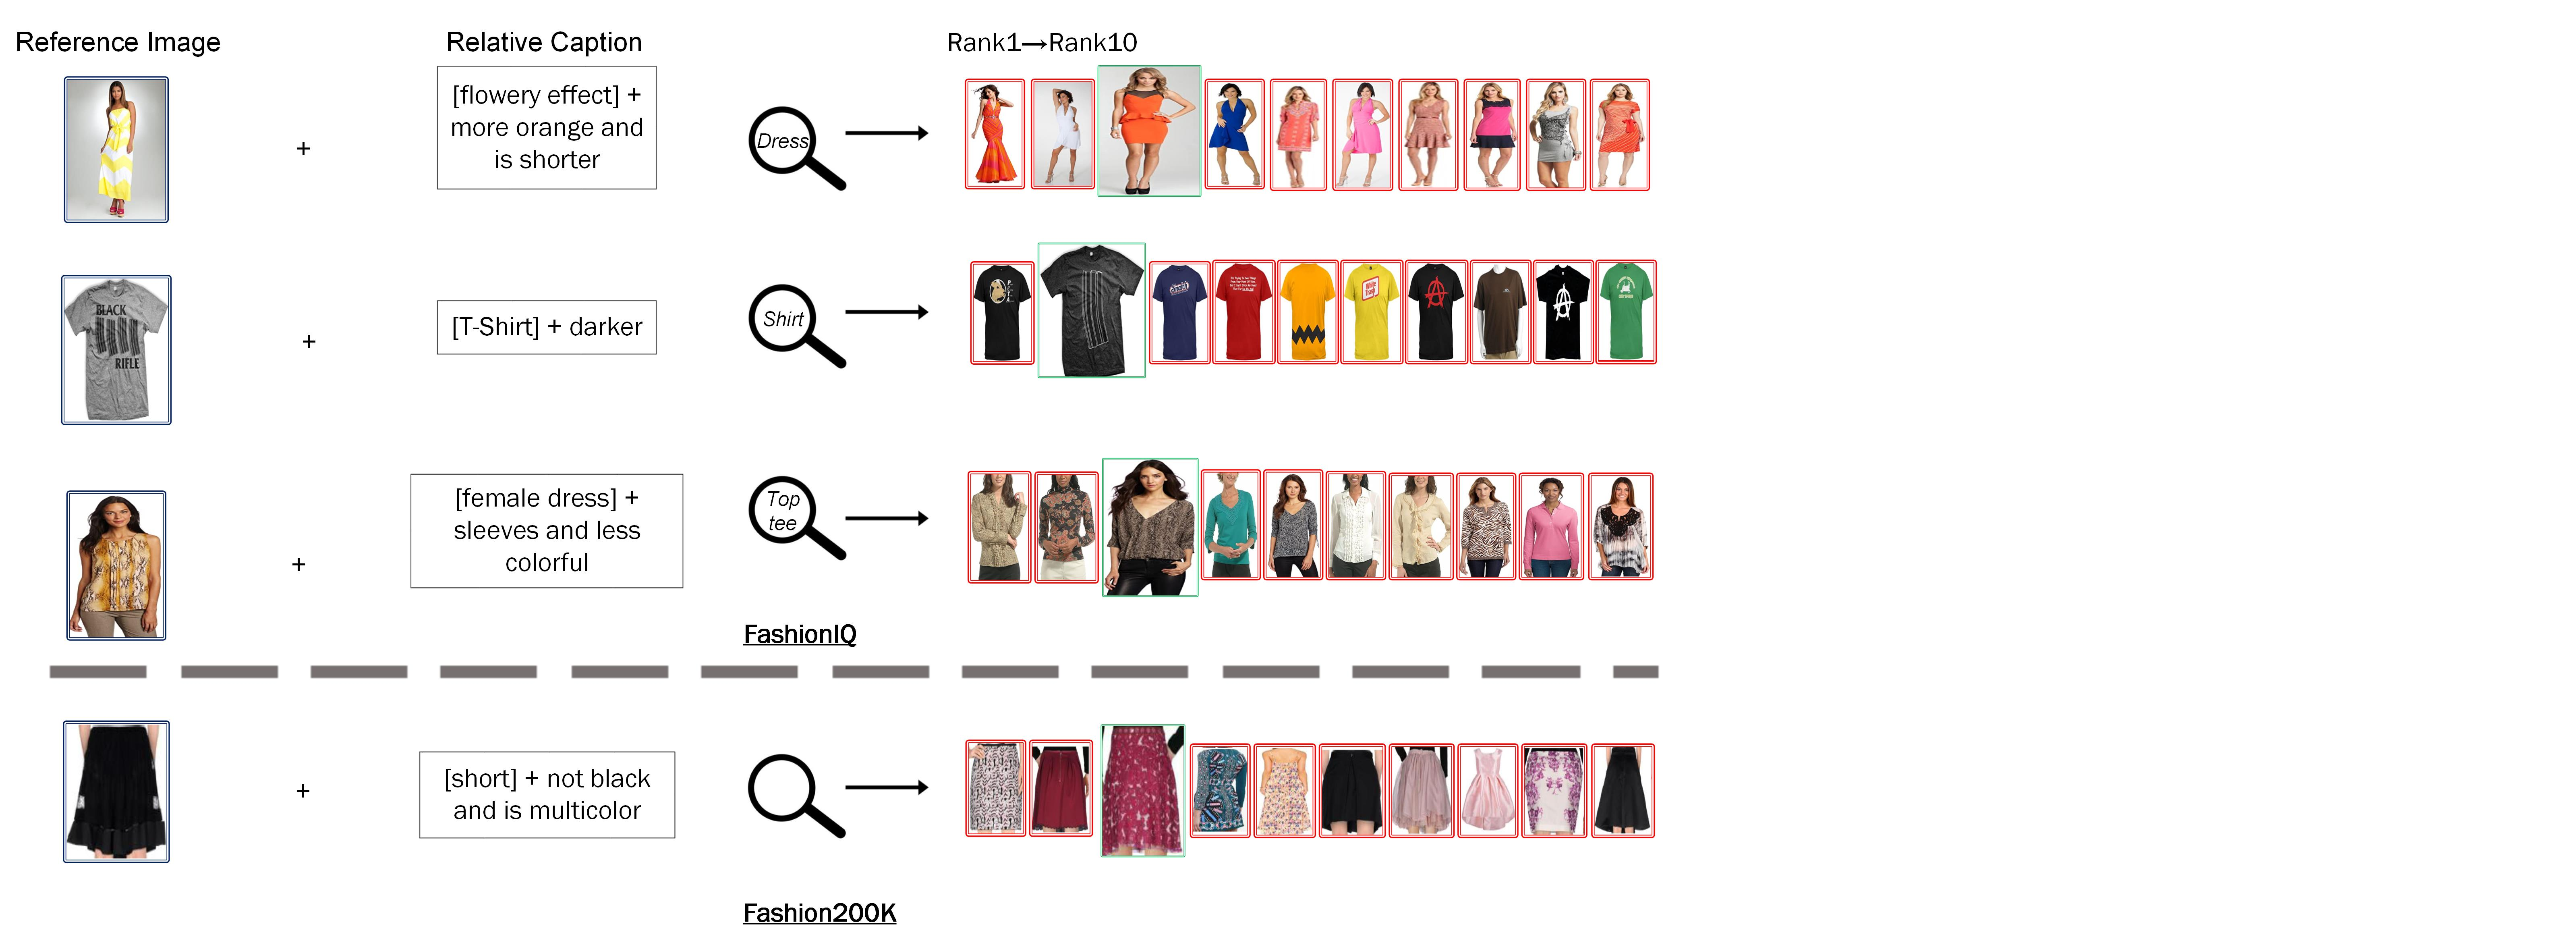
\includegraphics[width=1.5\textwidth,height=75mm]{QR.jpg}
     \caption{Qualitative Retrieval Examples from Fashion-IQ and Fashion-200K Datasets During Inference Stage: Query Image with [KES Pseudo Word Tokens] and Text Query (in Black) on the Left, Top-10 Retrieved Images Ranked by Descending Similarity Scores (Recall@10) on the Right; Target Image Surrounded by a Green Border and Enhanced Visualization, Non-Target Images Framed in Red}
    \label{fig:QR}
\end{figure*}
\FloatBarrier

\section{Ablation Studies}\label{sec:Ablation_studies}
\subsection*{Wholesome and Individual modality CLIP Alignment}\label{sec:joint_encoders}
We present a series of experiments that demonstrate how wholesome CLIP alignment and individual encoder based alignment for specific tasks, contribute enhanced retrieval performance. For these experimentation, we utilize ResNet-50 based CLIP encoder. The performance outcomes for Fashion-IQ, Fashion-200K, and CIRR are detailed in Table-\ref{tab:fashioniq_encoders}, Table-\ref{tab:Fashion200_encoders}, and Table-\ref{tab:CIRR_encoders}, accordingly. 

\par Remarkably, the simple element-wise summation of CLIP features without any domain-specific training yields impressive results on Fashion-IQ, Fashion-200K, and CIRR. The observed results are particularly noteworthy as they highlight that the CLIP visio-linguistic shared features scheme possesses strong additive properties, despite the training goal not being directly centered on this characteristic. Using only $\mathcal{E}_i$ results in a significant performance boost compared to the original CLIP features. Utilizing solely $\mathcal{E}_i$ leads to a significant performance boost compared to the original CLIP features, and such an improvement is expected, particularly if summation is employed as the combination function. Nevertheless, the greatest enhancement is observed upon employing the trained relational network.
Fine-tuning of $\mathcal{E}_t$ slightly leads to better performance than fine-tuning of $\mathcal{E}_i$.
\par The optimal results on both the datasets are attained when both encoders are fine-tuned. The summation of these fine-tuned features surpasses the performance of combining generic CLIP features with the relational network by a substantial margin.
Furthermore, when combining features of the joint query with the relational network, performance is further enhanced.

% \begin{table}[]
\begin{table}[htbp!]
\centering
\begin{tabular}{|c|c|c|c|c|c|c|c|c|}
    \hline
    Embd&$\mathcal{E}_i$& $\mathcal{E}_t$ & \multicolumn{2}{c|}{Dress} & \multicolumn{2}{c|}{Shirt} & \multicolumn{2}{c|}{Toptee} \\    \hline
    \multicolumn{3}{|c|}{} & Recall@10 & Recall@50 & Recall@10 & Recall@50 & Recall@10 & Recall@50 \\    \hline
    {\begin{tabular}{@{}c@{}}\\\emph{SUM}\end{tabular}} &$\times$&$\times$&16.73  & 35.64& 18.52& 34.86& 21.78& 41.36\\
     &\checkmark&$\times$&29.45  &  51.86 & 29.68& 51.38& 33.89& 56.87\\
     &$\times$&$\checkmark$&28.01 &  52.36 & 33.48& 52.98& 34.98& 59.78\\
     &\checkmark&$\checkmark$&35.49  &  68.58 & 39.45& 57.28& 43.68& 66.58\\
    \hline
    {\emph{RN}} &$\times$&$\times$&26.85  & 52.68& 32.07& 51.26& 31.80& 57.57\\
     &\checkmark&$\times$&32.84  &  55.48 & 34.12& 54.68& 37.35& 62.36\\
     &$\times$&$\checkmark$&30.98  &  53.78 & 35.89& 56.69& 37.20& 63.22\\
     &\checkmark&$\checkmark$&36.75  &  62.19 & 38.49& 59.87& 44.88& 68.59\\
    \hline
\end{tabular}
\caption{Recall@K for FashionIQ dataset when using summation and relational network for amalgation of CLIP generated embeddings. Moreover, exploring the effect of wholesome CLIP alignment and individual encoder effect}
\label{tab:fashioniq_encoders}
\end{table}


\begin{table}[htbp!]
\centering
\begin{tabular}{|c|c|c|cccc|}
\hline
\multicolumn{1}{|c|}{Embd}              & $\mathcal{E}_i$ & $\mathcal{E}_t$ & \multicolumn{4}{c|}{Fashion-200K} \\ \hline
                                           &    &    & \multicolumn{1}{l|}{Recall@1}   & \multicolumn{1}{l|}{Recall@5}   & \multicolumn{1}{l|}{Recall@10}  & Recall@50  \\ \hline
\multicolumn{1}{|c|}{{\emph{SUM}}} &  $\times$  & $\times$   & \multicolumn{1}{l|}{20.35} & \multicolumn{1}{l|}{29.83} & \multicolumn{1}{l|}{41.95} & 66.21 \\  
\multicolumn{1}{|c|}{}                     & \checkmark   &  $\times$  & \multicolumn{1}{l|}{30.23} & \multicolumn{1}{l|}{35.19} & \multicolumn{1}{l|}{48.53} & 70.35 \\  
\multicolumn{1}{|c|}{}                     & $\times$   &  \checkmark  & \multicolumn{1}{l|}{32.60} & \multicolumn{1}{l|}{37.30} & \multicolumn{1}{l|}{48.32} & 69.63 \\  
\multicolumn{1}{|c|}{}                     &  \checkmark  & \checkmark   & \multicolumn{1}{l|}{39.45} & \multicolumn{1}{l|}{43.46} & \multicolumn{1}{l|}{54.17} & 72.32 \\ \hline
{\emph{RN}}   & $\times$   &  $\times$  & \multicolumn{1}{l|}{30.23} & \multicolumn{1}{l|}{33.72} & \multicolumn{1}{l|}{46.23} & 63.29 \\  
                                           &  \checkmark  &  $\times$  & \multicolumn{1}{l|}{33.96} & \multicolumn{1}{l|}{38.29} & \multicolumn{1}{l|}{50.79} & 64.08 \\  
                                           &  $\times$  &  \checkmark  & \multicolumn{1}{l|}{35.29} & \multicolumn{1}{l|}{41.30} & \multicolumn{1}{l|}{52.30} & 71.32 \\  
                                           & \checkmark   &  \checkmark  & \multicolumn{1}{l|}{41.06} & \multicolumn{1}{l|}{45.26} & \multicolumn{1}{l|}{59.91} & 79.36 \\ \hline
\end{tabular}
\caption{Recall@K for Fashion200K dataset when using summation and relational network for amalgation of CLIP generated embeddings. Moreover, Exploring, the effect of wholesome CLIP alignment and individual encoder effect}
\label{tab:Fashion200_encoders}
\end{table}

\begin{table}[!htbp]
\centering
\begin{tabular}{|c|c|c|ccc|}
\hline
\multicolumn{1}{|c|}{Embd}              & $\mathcal{E}_i$ & $\mathcal{E}_t$ & \multicolumn{3}{c|}{CIRR} \\ \hline
                                           &    &    & \multicolumn{1}{l|}{Recall@5}   & \multicolumn{1}{l|}{Recall@10}  & Recall@50  \\ \hline
\multicolumn{1}{|c|}{{\emph{SUM}}} &  $\times$  & $\times$   &\multicolumn{1}{l|}{30.25} & \multicolumn{1}{l|}{43.76} & 64.58 \\  
\multicolumn{1}{|c|}{}                     & {\checkmark}   &  $\times$  & \multicolumn{1}{l|}{36.32} & \multicolumn{1}{l|}{49.60} & 69.89 \\  
\multicolumn{1}{|c|}{}                     & $\times$   &  {\checkmark}  & \multicolumn{1}{l|}{39.56} & \multicolumn{1}{l|}{51.68} & 70.49 \\  
\multicolumn{1}{|c|}{}                     &  {\checkmark}  & {\checkmark}   & \multicolumn{1}{l|}{42.68} & \multicolumn{1}{l|}{55.98} & 76.23 \\ \hline
{\emph{RN}}   & $\times$   &  $\times$  & \multicolumn{1}{l|}{35.24} & \multicolumn{1}{l|}{56.38} & 69.56 \\  
&  {\checkmark}  &  $\times$  & \multicolumn{1}{l|}{41.25} & \multicolumn{1}{l|}{63.78} & 73.58 \\  
&  $\times$  &  {\checkmark}   & \multicolumn{1}{l|}{46.85} & \multicolumn{1}{l|}{71.57} & 83.68 \\  
& {\checkmark}   &  {\checkmark}  & \multicolumn{1}{l|}{59.23} & \multicolumn{1}{l|}{82.74} & 91.89 \\ \hline
\end{tabular}
\caption{Recall@K for CIRR dataset when using summation and relational network for amalgamation of CLIP-generated embeddings. Moreover, exploring the effect of wholesome CLIP alignment and individual encoder effect}
\label{tab:CIRR_encoders}
\end{table}
% \vspace{-50mm}
\FloatBarrier

\subsection*{Joint Vs Sequential training approach}
We also examined the effect of joint and sequential training of CLIP encoders and relational network. The experimental procedure involved two cases: First, joint training in which CLIP encoders are simultaneously trained with relational network, and second, following the proposed approach. In both scenarios, fine-tuning of the $\mathcal{E}_i$ or $\mathcal{E}_t$ was enabled, either separately or jointly same as discussed in section \ref{sec:joint_encoders}. The findings of this ablation study are outlined in Table \ref{tab:fashioniq_joint_seq}, Table \ref{tab:Fashion200_joint_seq} and Table \ref{tab:CIRR_joint_seq} for FashionIQ, Fashion200K and CIRR datasets respectively. The Sequential training approach consistently outperforms the joint approach on all three datasets.

These results offer support for the efficacy of establishing an embedding scheme with strong additive properties. The hypothesis proposes that when the relational network is trained together with the CLIP encoders in a joint manner, the system faces difficulties in learning both the combined embedding structure and the fusion function in a unified way. Consequently, this challenge hinders the system's performance, leading to suboptimal results.

\begin{table}[!htbp]
\centering
\begin{tabular}{|c|c|c|c|c|c|c|c|c|}
    \hline
    Training&$\mathcal{E}_i$& $\mathcal{E}_t$ & \multicolumn{2}{c|}{Dress} & \multicolumn{2}{c|}{Shirt} & \multicolumn{2}{c|}{Toptee} \\    \hline
    \multicolumn{3}{|c|}{} & Recall@10 & Recall@50 & Recall@10 & Recall@50 & Recall@10 & Recall@50 \\    \hline
    {\emph{Jointly}} &$\checkmark$&$\times$&30.29  & 53.49& 31.79& 53.14& 33.55& 59.15\\
     &$\times$&$\checkmark$&30.19  &  53.64 & 33.02& 54.41& 35.90& 61.60\\
     &$\checkmark$&$\checkmark$&34.65 &  60.83 & 37.29& 59.02& 41.20& 65.99\\ \hline
    {\emph{Sequentially}} &\checkmark&$\times$&32.84  &  55.48 & 34.12& 54.68& 37.35& 62.36\\
     &$\times$&$\checkmark$&30.98  &  53.78 & 35.89& 56.69& 37.20& 63.22\\
     &\checkmark&$\checkmark$&36.75  &  62.19 & 38.49& 59.87& 44.88& 68.59\\  \hline
\end{tabular}
\caption{Joint Vs Sequential training approach for FashionIQ dataset}
\label{tab:fashioniq_joint_seq}
\end{table}


\begin{table}[!htbp]
\centering
\begin{tabular}{|l|l|l|llll|}
\hline
\multicolumn{1}{|c|}{Training}              & $\mathcal{E}_i$ & $\mathcal{E}_t$ & \multicolumn{4}{c|}{Fashion-200K} \\ \hline
                                           &    &    & \multicolumn{1}{l|}{Recall@1}   & \multicolumn{1}{l|}{Recall@5}   & \multicolumn{1}{l|}{Recall@10}  & Recall@50  \\ \hline
\multicolumn{1}{|c|}{{\emph{Jointly}}} &\checkmark   &  $\times$  & \multicolumn{1}{l|}{31.56} & \multicolumn{1}{l|}{33.28} & \multicolumn{1}{l|}{56.68} & 52.38 \\  
\multicolumn{1}{|c|}{}                     & $\times$   &  \checkmark  & \multicolumn{1}{l|}{33.47} & \multicolumn{1}{l|}{36.93} & \multicolumn{1}{l|}{57.45} & 51.19 \\  
\multicolumn{1}{|c|}{}                     &  \checkmark  & \checkmark   & \multicolumn{1}{l|}{37.38} & \multicolumn{1}{l|}{40.26} & \multicolumn{1}{l|}{58.29} & 55.38\\ \hline
{\emph{Sequentially}}       &  \checkmark  &  $\times$  & \multicolumn{1}{l|}{33.96} & \multicolumn{1}{l|}{38.29} & \multicolumn{1}{l|}{50.79} & 64.08 \\  
&  $\times$  &  \checkmark  & \multicolumn{1}{l|}{35.29} & \multicolumn{1}{l|}{41.30} & \multicolumn{1}{l|}{52.30} & 71.32 \\  
& \checkmark   &  \checkmark  & \multicolumn{1}{l|}{41.06} & \multicolumn{1}{l|}{45.26} & \multicolumn{1}{l|}{59.91} & 79.36 \\ \hline
\end{tabular}
\caption{Joint Vs Sequential training approach for Fashion200K dataset}
\label{tab:Fashion200_joint_seq}
\end{table}


\begin{table}[!htbp]
\centering
\begin{tabular}{|l|l|l|lll|}
\hline
\multicolumn{1}{|c|}{Training}              & $\mathcal{E}_i$ & $\mathcal{E}_t$ & \multicolumn{3}{c|}{CIRR} \\ \hline
&    &    & \multicolumn{1}{l|}{Recall@5}   & \multicolumn{1}{l|}{Recall@10}  & Recall@50  \\ \hline
\multicolumn{1}{|c|}{{\emph{Jointly}}} & {\checkmark}   &  $\times$  & \multicolumn{1}{l|}{54.98} & \multicolumn{1}{l|}{69.28} & 79.63 \\  
\multicolumn{1}{|c|}{}                     & $\times$   &  {\checkmark}  & \multicolumn{1}{l|}{55.27} & \multicolumn{1}{l|}{68.59} & 80.25 \\  
\multicolumn{1}{|c|}{}                     &  {\checkmark}  & {\checkmark}   & \multicolumn{1}{l|}{57.14} & \multicolumn{1}{l|}{79.25} & 89.36\\ \hline
{\emph{Sequentially}}       &  {\checkmark}  &  $\times$  & \multicolumn{1}{l|}{50.69} & \multicolumn{1}{l|}{75.28} & 80.19 \\  
&  $\times$  &  {\checkmark}  & \multicolumn{1}{l|}{51.23} & \multicolumn{1}{l|}{76.58} & 81.63 \\  
& {\checkmark}   &  {\checkmark}  & \multicolumn{1}{l|}{59.23} & \multicolumn{1}{l|}{82.74} & 91.89 \\ \hline
\end{tabular}
\caption{Joint Vs Sequential training approach for CIRR dataset}
\label{tab:CIRR_joint_seq}
\end{table}



\section{Conclusion and future work}\label{sec:conclusion}
In this research work, we have introduced an innovative alignment scheme crafted to tailor visual linguistic frameworks for CBIR. The primary aim is to alleviate the mismatch between both modalities and the downstream task of image retrieval, utilizing composed representation to enhance the additive nature of the embedding plans. Prior to composed representation textual modality has been improved through Knowledge Embedded Stream. Subsequently, we propose a relational network in the second stage, facilitating a meaningful fusion of aligned multimodal features. We conduct our experiments on the demanding fashion domain datasets i.e.; Fashion-IQ \& Fashion-200K, in addition to the CIRR dataset, which includes real-world images. The experimental findings demonstrate that our approach significantly outperforms existing cutting-edge methods. Additionally, ablation studies were performed to evaluate the performance of various versions of the suggested method, concluding that sequentially training both stages yields superior results across all metrics.

The conducted experiments investigate the effect of our suggested method on the feature distribution within the embedding scheme, as well as the impact of modifying these embeddings on the effectiveness of retrieval. In upcoming research, we aim to explore new techniques for extracting image features, such as leveraging vision transformers in encoder-decoder architectures, along with incorporating text feature embeddings. \\

\textbf{Conflict of interest/Competing interests:} The authors declare that they have no known competing financial interests or personal relationships that could have appeared to influence the work reported in this paper.

% \bibliographystyle{ieeetr} 
\bibliography{References}

\end{document}